\documentclass[11pt, a4paper]{article}

% ── 패키지 ──
\usepackage{fontspec}
\usepackage{xeCJK}
\xeCJKsetup{CJKspace=true}
\setCJKmainfont{AppleSDGothicNeo-Regular}[
  BoldFont=AppleSDGothicNeo-Bold,
]
\setCJKsansfont{AppleSDGothicNeo-Regular}[
  BoldFont=AppleSDGothicNeo-Bold,
]
\usepackage[margin=2.5cm]{geometry}
\usepackage{graphicx}
\usepackage{xcolor}
\usepackage{hyperref}
\usepackage{fancyhdr}
\usepackage{titlesec}
\usepackage{enumitem}
\usepackage{tcolorbox}
\usepackage{booktabs}
\usepackage{multirow}
\usepackage{float}
\usepackage{caption}
\usepackage{subcaption}
\usepackage{setspace}

% ── 색상 정의 ──
\definecolor{eduprimary}{HTML}{5B51F6}
\definecolor{edudark}{HTML}{1E1B3A}
\definecolor{edugray}{HTML}{6B7280}
\definecolor{edulightbg}{HTML}{F8F9FB}
\definecolor{edusuccess}{HTML}{10B981}
\definecolor{eduwarning}{HTML}{F59E0B}
\definecolor{edudanger}{HTML}{EF4444}

% ── 하이퍼링크 설정 ──
\hypersetup{
  colorlinks=true,
  linkcolor=eduprimary,
  urlcolor=eduprimary,
  pdftitle={EduOps 사용 설명서},
  pdfauthor={EduOps Team},
}

% ── 헤더/푸터 ──
\pagestyle{fancy}
\fancyhf{}
\fancyhead[L]{\small\color{edugray}EduOps 사용 설명서}
\fancyhead[R]{\small\color{edugray}v1.0}
\fancyfoot[C]{\small\color{edugray}\thepage}
\renewcommand{\headrulewidth}{0.4pt}

% ── 섹션 스타일 ──
\titleformat{\section}
  {\Large\bfseries\color{edudark}}
  {\thesection}{1em}{}
  [\vspace{-0.5em}\color{eduprimary}\rule{\textwidth}{1.5pt}]

\titleformat{\subsection}
  {\large\bfseries\color{edudark}}
  {\thesubsection}{1em}{}

\titleformat{\subsubsection}
  {\normalsize\bfseries\color{edudark}}
  {\thesubsubsection}{1em}{}

% ── 팁 박스 ──
\newtcolorbox{tipbox}{
  colback=eduprimary!5,
  colframe=eduprimary,
  fonttitle=\bfseries,
  title={\small TIP},
  boxrule=0.5pt,
  arc=4pt,
  left=8pt, right=8pt, top=4pt, bottom=4pt,
}

\newtcolorbox{warningbox}{
  colback=eduwarning!8,
  colframe=eduwarning,
  fonttitle=\bfseries,
  title={\small 주의},
  boxrule=0.5pt,
  arc=4pt,
  left=8pt, right=8pt, top=4pt, bottom=4pt,
}

\newtcolorbox{notebox}{
  colback=edulightbg,
  colframe=edugray!50,
  boxrule=0.5pt,
  arc=4pt,
  left=8pt, right=8pt, top=4pt, bottom=4pt,
}

% ── 스크린샷 명령어 ──
\newcommand{\screenshot}[3][1.0]{%
  \begin{figure}[H]
    \centering
    \includegraphics[width=#1\textwidth]{screenshots/#2}
    \caption{#3}
    \label{fig:#2}
  \end{figure}
}

% ── 메뉴 경로 표시 ──
\newcommand{\menu}[1]{\textcolor{eduprimary}{\textbf{#1}}}
\newcommand{\btn}[1]{\colorbox{eduprimary!10}{\textcolor{eduprimary}{\textbf{#1}}}}

% ══════════════════════════════════════════════
\begin{document}

% ── 표지 ──
\begin{titlepage}
  \begin{center}
    \vspace*{3cm}

    {\Huge\bfseries\color{edudark} EduOps}\\[0.3cm]
    {\Large\color{eduprimary} 종합학원 관리 시스템}\\[1.5cm]

    {\LARGE\bfseries 사용 설명서}\\[0.5cm]
    {\large User Manual v1.0}\\[3cm]

    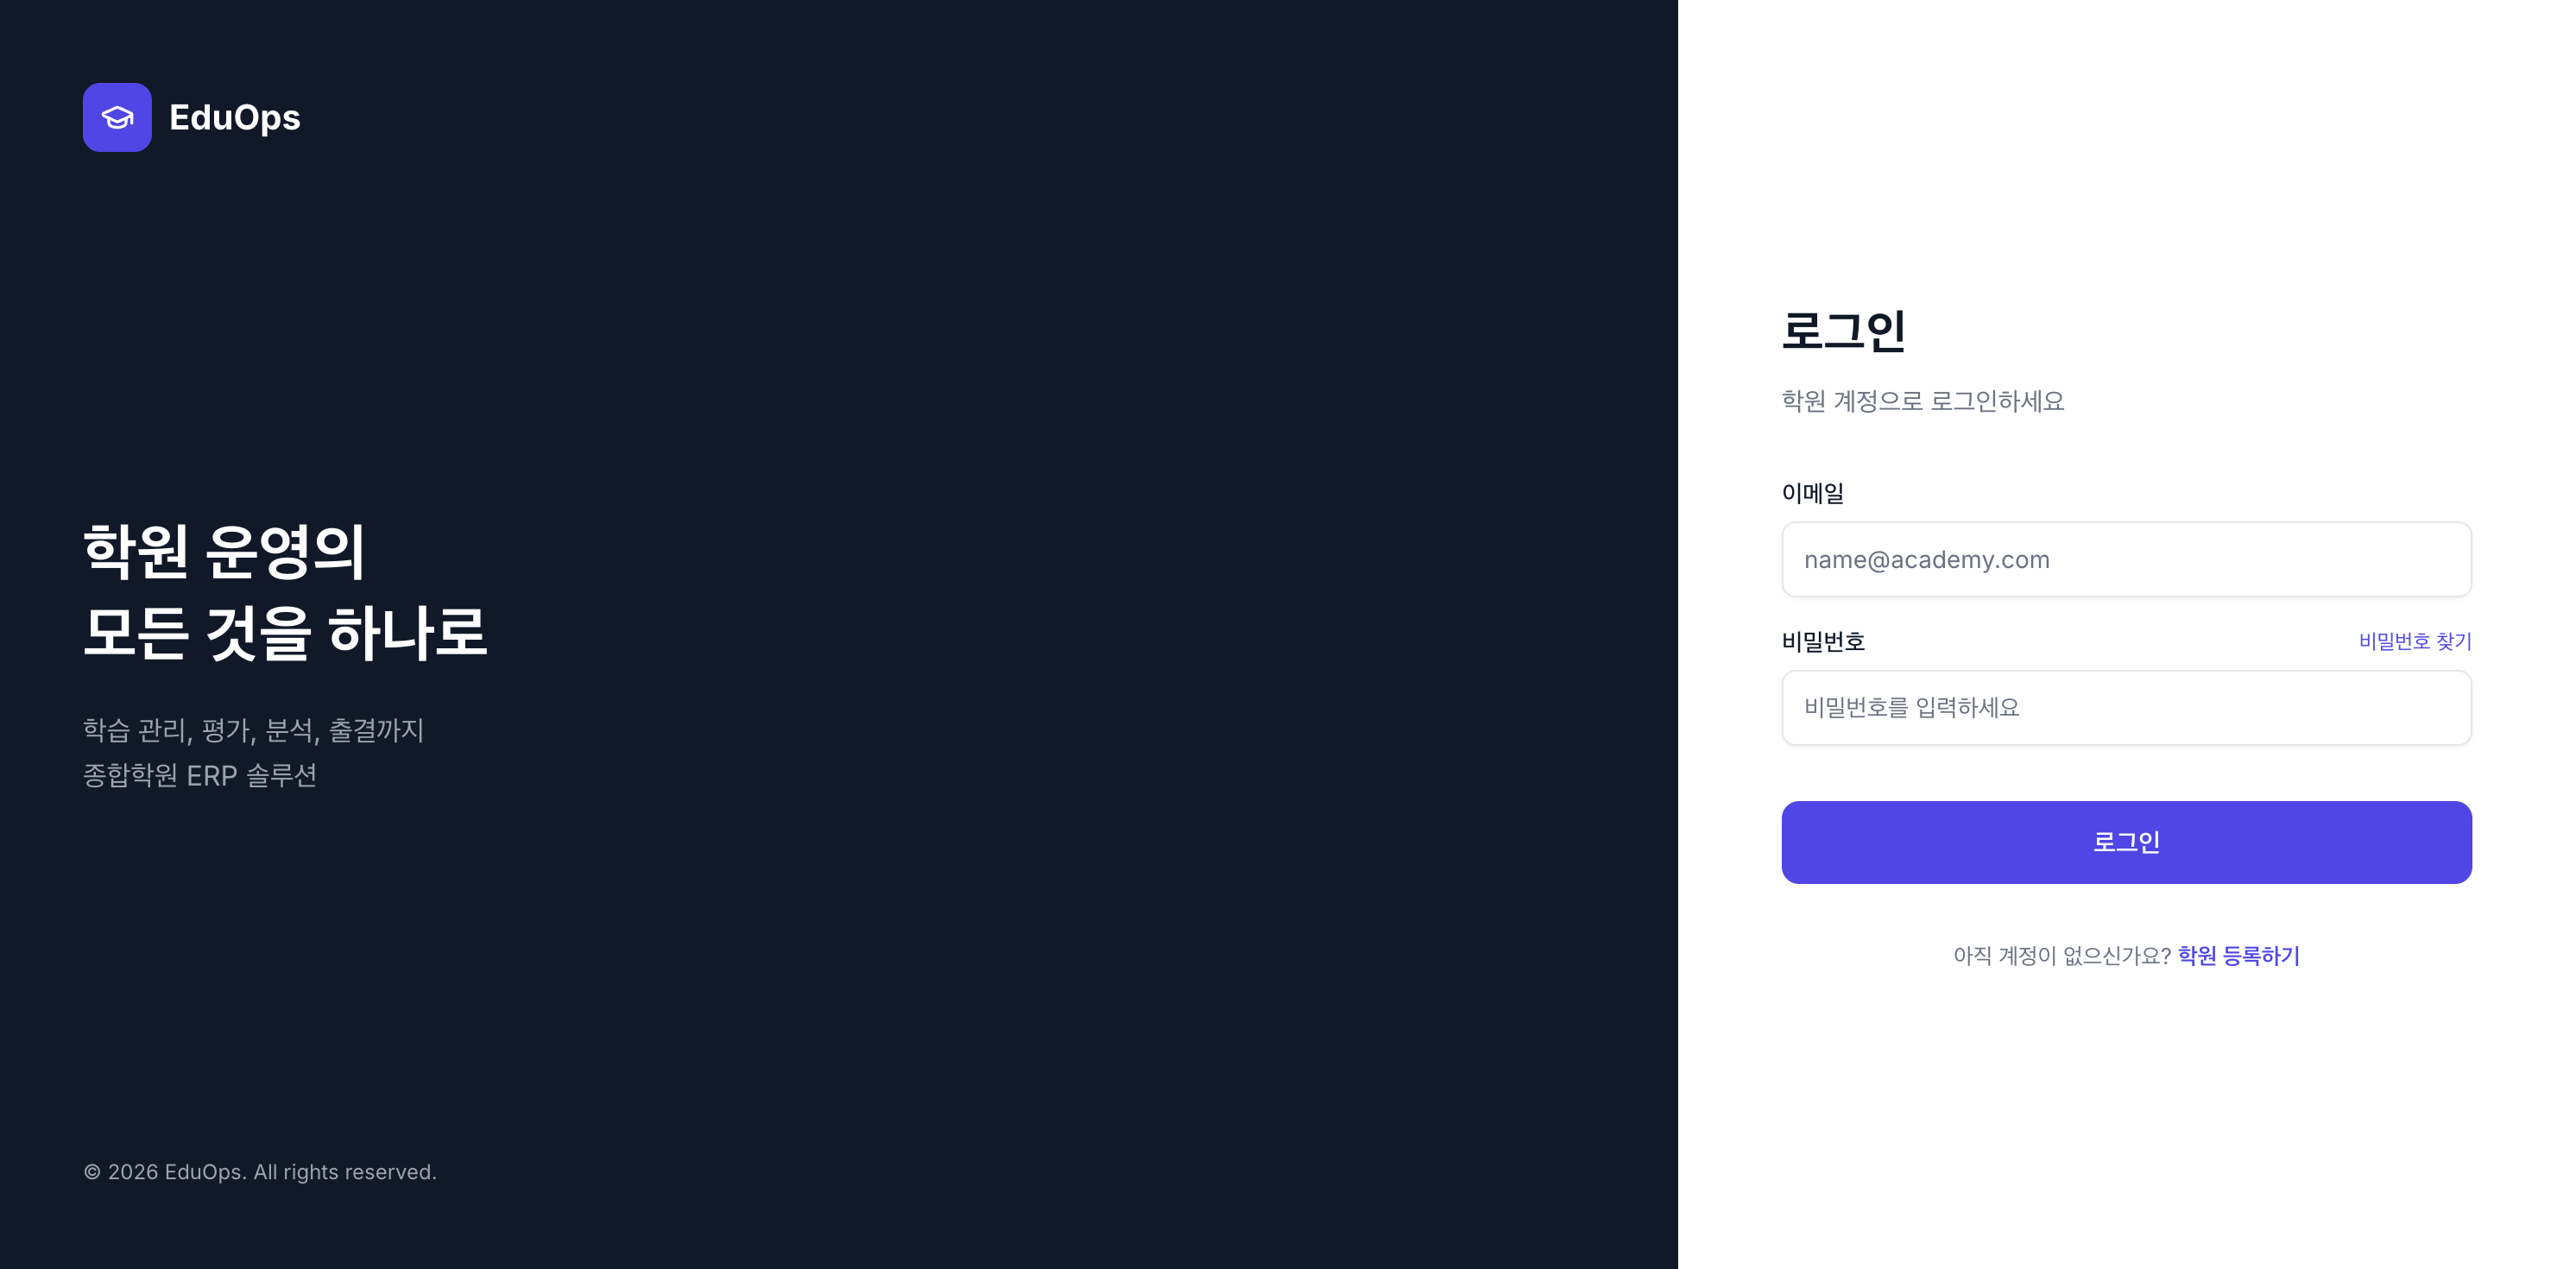
\includegraphics[width=0.85\textwidth]{screenshots/01_login.png}\\[2cm]

    {\large\color{edugray}
    학습 관리 $\cdot$ 평가 $\cdot$ 분석 $\cdot$ 출결 $\cdot$ 수납\\[0.3cm]
    학원 운영의 모든 것을 하나로}\\[2cm]

    {\normalsize 2026년 3월}\\[0.5cm]
    {\small\color{edugray} \textcopyright\ 2026 EduOps. All rights reserved.}
  \end{center}
\end{titlepage}

% ── 목차 ──
\tableofcontents
\newpage

% ══════════════════════════════════════════════
\section{시작하기}
% ══════════════════════════════════════════════

EduOps는 학원 운영에 필요한 학생 관리, 반 편성, 출결, 평가, 성적 분석, 수납까지
모든 기능을 하나의 웹 시스템으로 통합한 \textbf{종합학원 ERP 솔루션}입니다.

\subsection{시스템 요구사항}

\begin{itemize}[leftmargin=1.5em]
  \item \textbf{브라우저}: Chrome, Safari, Edge, Firefox 최신 버전
  \item \textbf{디바이스}: PC, 태블릿, 모바일 (반응형 지원)
  \item \textbf{인터넷}: 안정적인 인터넷 연결 필요
\end{itemize}

\subsection{회원가입 (학원 등록)}

EduOps를 처음 사용하려면 학원 계정을 등록해야 합니다.

\begin{enumerate}[leftmargin=1.5em]
  \item 로그인 화면 하단의 \btn{학원 등록하기} 링크를 클릭합니다.
  \item 다음 정보를 입력합니다:
    \begin{itemize}
      \item \textbf{학원명}: 학원의 공식 명칭
      \item \textbf{원장 이름}: 관리자 이름
      \item \textbf{이메일}: 로그인에 사용할 이메일 주소
      \item \textbf{비밀번호}: 6자 이상의 비밀번호
      \item \textbf{전화번호}: 학원 대표 연락처 (선택)
    \end{itemize}
  \item \btn{학원 등록} 버튼을 클릭하면 계정이 생성되고 대시보드로 이동합니다.
\end{enumerate}

\begin{tipbox}
  가입 시 입력한 이메일로 인증 메일이 발송될 수 있습니다. 메일함을 확인해주세요.
\end{tipbox}

\subsection{로그인}

\screenshot[0.85]{01_login.png}{EduOps 로그인 화면}

\begin{enumerate}[leftmargin=1.5em]
  \item 접속 주소로 이동합니다.
  \item \textbf{이메일}과 \textbf{비밀번호}를 입력합니다.
  \item \btn{로그인} 버튼을 클릭합니다.
\end{enumerate}

비밀번호를 분실한 경우, \menu{비밀번호 찾기}를 클릭하여 이메일로 재설정 링크를 받을 수 있습니다.


% ══════════════════════════════════════════════
\section{대시보드}
% ══════════════════════════════════════════════

로그인 후 가장 먼저 보이는 화면입니다. 학원 운영 현황을 한눈에 파악할 수 있습니다.

\screenshot[0.95]{02_dashboard.png}{대시보드 메인 화면}

대시보드는 다음 정보를 요약해서 보여줍니다:

\begin{itemize}[leftmargin=1.5em]
  \item \textbf{전체 학생}: 현재 재원생 수
  \item \textbf{운영 과목}: 등록된 과목 수와 과목명
  \item \textbf{이번달 평가}: 이번 달에 진행된/예정된 평가 건수
  \item \textbf{전체 평균}: 이번 달 평가 전체 평균 점수
  \item \textbf{최근 평가}: 최근 평가 목록과 평균 점수 (클릭하면 상세 페이지로 이동)
  \item \textbf{오늘의 출결}: 당일 출결 현황
  \item \textbf{교재별 진도율}: 교재별 학습 진행률
\end{itemize}

\begin{tipbox}
  각 카드의 \menu{전체 보기 →} 링크를 클릭하면 해당 관리 페이지로 바로 이동합니다.
\end{tipbox}

\subsection{사이드바 네비게이션}

화면 왼쪽의 사이드바를 통해 모든 기능에 접근할 수 있습니다.

\begin{table}[H]
\centering
\begin{tabular}{lll}
\toprule
\textbf{카테고리} & \textbf{메뉴} & \textbf{설명} \\
\midrule
\multirow{1}{*}{---} & 대시보드 & 학원 현황 요약 \\
\midrule
\multirow{3}{*}{학습 관리} & 과목 관리 & 과목 등록/수정/학생 배정 \\
                          & 교재/단원 & 교재 등록, 단원 진도 관리 \\
                          & 평가 관리 & 시험/퀴즈 등록 및 관리 \\
\midrule
\multirow{2}{*}{관리} & 학생 관리 & 학생 정보 CRUD \\
                      & 반 관리 & 반 편성, 학생 배정 \\
\midrule
\multirow{2}{*}{성적/분석} & 성적 관리 & 평가별 성적 입력 \\
                          & 분석/리포트 & 학생별 성적 추이 분석 \\
\midrule
\multirow{3}{*}{운영} & 출결 관리 & 출석/지각/결석 기록 \\
                      & 과제 관리 & 과제 등록, 제출 현황 \\
                      & 수납 관리 & 학원비 수납 현황 관리 \\
\midrule
\multirow{1}{*}{---} & 설정 & 학원 정보 수정 \\
\bottomrule
\end{tabular}
\caption{사이드바 메뉴 구성}
\end{table}


% ══════════════════════════════════════════════
\section{학생 관리}
% ══════════════════════════════════════════════

학원에 등록된 학생들의 정보를 관리하는 페이지입니다.

\screenshot[0.95]{03_students.png}{학생 관리 화면}

\subsection{학생 목록}

학생 관리 페이지에서는 다음 정보를 확인할 수 있습니다:
\begin{itemize}[leftmargin=1.5em]
  \item \textbf{이름}: 학생의 이름 (클릭하면 상세 페이지로 이동)
  \item \textbf{학교/학년}: 재학 중인 학교와 학년
  \item \textbf{수강 과목}: 수강 중인 과목 태그
  \item \textbf{상태}: 재원/퇴원 상태
\end{itemize}

상단의 \textbf{검색창}, \textbf{과목 필터}, \textbf{상태 필터}를 활용하여
원하는 학생을 빠르게 찾을 수 있습니다.

\subsection{학생 추가}

\begin{enumerate}[leftmargin=1.5em]
  \item 우측 상단의 \btn{+ 학생 추가} 버튼을 클릭합니다.
  \item 학생 정보를 입력합니다:
    \begin{itemize}
      \item 이름 (필수), 영어 이름
      \item 학교, 학년
      \item 학부모 연락처, 학생 연락처
      \item 메모
    \end{itemize}
  \item \btn{저장} 버튼을 클릭하여 등록을 완료합니다.
\end{enumerate}

\subsection{학생 상세}

학생 이름을 클릭하면 해당 학생의 상세 페이지로 이동합니다. 상세 페이지에서는:

\begin{itemize}[leftmargin=1.5em]
  \item 학생 기본 정보 수정
  \item 수강 과목 확인
  \item 출결 이력 조회
  \item 평가 성적 이력 확인
  \item 과제 제출 현황 확인
\end{itemize}


% ══════════════════════════════════════════════
\section{반 관리}
% ══════════════════════════════════════════════

반을 생성하고, 학생을 배정하여 수업을 체계적으로 운영할 수 있습니다.

\screenshot[0.95]{04_classes.png}{반 관리 화면}

\subsection{반 목록}

등록된 반이 카드 형태로 표시됩니다. 각 카드에는 반 이름, 담당 과목, 학생 수가 표시되며, 클릭하면 반 상세 화면으로 이동합니다.

\subsection{반 생성}

\begin{enumerate}[leftmargin=1.5em]
  \item \btn{+ 반 추가} 버튼을 클릭합니다.
  \item 반 이름, 설명, 연결 과목을 입력합니다.
  \item 저장 후, 반 상세 화면에서 학생을 배정합니다.
\end{enumerate}

\subsection{반 상세 (클래스 허브)}

반 상세 화면은 해당 반의 모든 정보를 탭으로 구분하여 보여주는 \textbf{클래스 허브}입니다:

\begin{itemize}[leftmargin=1.5em]
  \item \textbf{개요 탭}: 학생 목록, 요약 통계, 교재 진도, 최근 평가
  \item \textbf{출결 탭}: 주간 출결 매트릭스 (학생 × 요일)
  \item \textbf{평가 탭}: 반 소속 학생의 평가 목록과 응시 현황
  \item \textbf{과제 탭}: 과제별 제출 현황과 마감일
  \item \textbf{수시기록 탭}: 단어시험, 숙제 등 일일 기록 입력 (스프레드시트 형태)
  \item \textbf{교재 탭}: 교재 연결/해제, 단원별 진도 관리
\end{itemize}

\begin{tipbox}
  반 상세 화면의 \btn{학부모 리포트} 버튼을 클릭하면 반 전체 학생의 학부모 리포트 링크를 한번에 생성할 수 있습니다. 생성된 링크를 카카오톡/문자로 공유하면 학부모가 로그인 없이 자녀의 학습 현황을 확인할 수 있습니다.
\end{tipbox}


% ══════════════════════════════════════════════
\section{과목 관리}
% ══════════════════════════════════════════════

학원에서 운영하는 과목을 등록하고 관리합니다.

\screenshot[0.95]{05_subjects.png}{과목 관리 화면}

\subsection{과목 카드}

각 과목은 카드 형태로 표시되며 다음 정보를 포함합니다:
\begin{itemize}[leftmargin=1.5em]
  \item 과목명 및 구분 색상
  \item 유형 (정규, 특강, 캠프, 수행평가, 프로젝트 등)
  \item 담당 강사
  \item 수강 학생 수
\end{itemize}

\subsection{과목 추가/수정}

\begin{enumerate}[leftmargin=1.5em]
  \item \btn{+ 과목 추가} 버튼 또는 과목명을 클릭합니다.
  \item 과목명, 유형, 담당 강사, 구분 색상을 설정합니다.
  \item 저장 후, \menu{학생 관리} 버튼으로 수강 학생을 배정합니다.
\end{enumerate}

\subsection{학생 배정}

과목 카드의 \menu{학생 관리} 버튼을 클릭하면 체크박스로 학생을 수강 등록/해제할 수 있습니다.
검색 기능을 활용하여 원하는 학생을 빠르게 찾을 수 있습니다.


% ══════════════════════════════════════════════
\section{교재/단원 관리}
% ══════════════════════════════════════════════

교재를 등록하고, 단원별 학습 진도를 추적합니다.

\screenshot[0.95]{06_textbooks.png}{교재/단원 관리 화면}

\subsection{화면 구성}

\begin{itemize}[leftmargin=1.5em]
  \item \textbf{좌측 패널}: 교재 목록. 과목 태그, 연도, 학년, 진도율이 표시됩니다.
  \item \textbf{우측 패널}: 선택된 교재의 단원 트리. 대단원/소단원 구조로 표시됩니다.
\end{itemize}

\subsection{교재 등록}

교재 관리 페이지 상단의 추가 버튼 또는 학원 관리 대시보드에서 교재를 등록합니다.
교재명, 과목, 학년, 연도를 입력하며, PDF 파일을 업로드하면 PDF 뷰어로도 확인 가능합니다.

\subsection{단원 진도 관리}

단원 트리에서 각 소단원의 상태를 클릭하여 변경할 수 있습니다:

\begin{itemize}[leftmargin=1.5em]
  \item \textcolor{edugray}{\textbf{미진행}}: 아직 학습하지 않은 단원
  \item \textcolor{eduprimary}{\textbf{진행중}}: 현재 학습 중인 단원
  \item \textcolor{edusuccess}{\textbf{완료}}: 학습이 완료된 단원
\end{itemize}

진도 변경 시 상단의 진도율 바가 자동으로 업데이트됩니다.


% ══════════════════════════════════════════════
\section{평가 관리}
% ══════════════════════════════════════════════

시험, 퀴즈, 수행평가 등을 등록하고 관리합니다.

\screenshot[0.95]{07_assessments.png}{평가 관리 화면}

\subsection{평가 목록}

등록된 평가가 테이블 형태로 표시됩니다:
\begin{itemize}[leftmargin=1.5em]
  \item 날짜, 과목, 평가명
  \item 유형 (시험/퀴즈/과제/수행평가/출석점수)
  \item 총점, 대상 학생 수
  \item 상태 (예정/진행중/완료)
\end{itemize}

과목 필터와 상태 필터로 원하는 평가를 검색할 수 있습니다.

\subsection{평가 등록}

\begin{enumerate}[leftmargin=1.5em]
  \item \btn{+ 평가 추가} 버튼을 클릭합니다.
  \item 평가명, 과목, 반, 유형, 날짜, 총점을 입력합니다.
  \item 저장하면 해당 반/과목의 학생들이 자동으로 대상자로 등록됩니다.
\end{enumerate}

\subsection{성적 입력}

평가를 클릭하면 성적 입력 화면으로 이동합니다. 학생별로 점수를 입력하고 저장합니다.


% ══════════════════════════════════════════════
\section{성적 관리}
% ══════════════════════════════════════════════

평가별 성적을 입력하고 조회하는 페이지입니다.

\screenshot[0.95]{08_scores.png}{성적 관리 화면}

평가 목록에서 평가를 선택하면 해당 평가의 학생별 성적을 입력하거나 수정할 수 있습니다.
반 필터를 활용하면 특정 반의 평가만 볼 수 있습니다.


% ══════════════════════════════════════════════
\section{출결 관리}
% ══════════════════════════════════════════════

학생의 출석, 지각, 결석, 인정결석을 기록하고 관리합니다.

\screenshot[0.95]{09_attendance.png}{출결 관리 화면}

\subsection{출결 기록}

\begin{enumerate}[leftmargin=1.5em]
  \item 날짜와 과목을 선택합니다.
  \item 학생 목록에서 각 학생의 출결 상태를 선택합니다:
    \begin{itemize}
      \item \textbf{O} 출석 \quad \textbf{△} 지각 \quad \textbf{X} 결석 \quad \textbf{◎} 인정결석
    \end{itemize}
  \item \btn{저장} 버튼을 클릭하여 기록을 저장합니다.
\end{enumerate}

\subsection{일괄 출결 등록}

\btn{일괄 등록} 기능을 사용하면 반 단위로 출결을 한 번에 등록할 수 있습니다.
날짜, 반, 과목을 선택하면 해당 반 학생이 자동으로 로드됩니다.


% ══════════════════════════════════════════════
\section{과제 관리}
% ══════════════════════════════════════════════

학생에게 과제를 부여하고, 제출 현황을 추적합니다.

\screenshot[0.95]{10_assignments.png}{과제 관리 화면}

\subsection{과제 등록}

\begin{enumerate}[leftmargin=1.5em]
  \item \btn{+ 과제 추가} 버튼을 클릭합니다.
  \item 과제 제목, 과목, 반, 마감일, 난이도를 입력합니다.
  \item 필수 여부를 설정하고, 대상 학생을 지정합니다.
  \item 저장하면 과제 목록에 추가됩니다.
\end{enumerate}

\subsection{제출 현황 확인}

과제를 클릭하면 학생별 제출 현황을 확인할 수 있습니다.
제출 상태(미제출/제출완료)를 변경하고, 제출일시가 자동으로 기록됩니다.


% ══════════════════════════════════════════════
\section{수납 관리}
% ══════════════════════════════════════════════

학원비 수납 현황을 관리하는 페이지입니다.

\screenshot[0.95]{11_payments.png}{수납 관리 화면}

\subsection{수납 현황 요약}

화면 상단에 해당 월의 수납 요약이 카드로 표시됩니다:
\begin{itemize}[leftmargin=1.5em]
  \item \textbf{총 청구액}: 해당 월 전체 청구 금액
  \item \textcolor{eduprimary}{\textbf{수납 완료}}: 납부가 완료된 금액
  \item \textcolor{eduwarning}{\textbf{미납}}: 아직 납부되지 않은 금액
  \item \textcolor{edudanger}{\textbf{연체}}: 납부기한이 지난 미납 금액
\end{itemize}

좌우 화살표로 월을 이동하여 과거/미래 수납 현황을 조회할 수 있습니다.

\subsection{수납 등록}

\begin{enumerate}[leftmargin=1.5em]
  \item \btn{+ 수납 등록} 버튼을 클릭합니다.
  \item 학생, 항목(예: 3월 수업료), 금액, 납부기한을 입력합니다.
  \item 메모를 추가할 수 있습니다 (선택).
  \item \btn{등록} 버튼을 클릭하여 수납 내역을 추가합니다.
\end{enumerate}

\subsection{반별 일괄 등록}

\begin{enumerate}[leftmargin=1.5em]
  \item \btn{반별 일괄 등록} 버튼을 클릭합니다.
  \item 반을 선택하면 해당 반의 전체 학생에게 동일한 수납 항목이 일괄 생성됩니다.
  \item 항목명, 금액, 납부기한을 입력합니다.
\end{enumerate}

\begin{tipbox}
  수납 목록에서 상태를 클릭하면 \textbf{미납 → 납부완료}로 변경할 수 있고, 수납 방법(현금/카드/이체)을 선택할 수 있습니다.
\end{tipbox}

\subsection{알림 문자 복사}

수납 내역의 액션 메뉴에서 \menu{알림 문자 복사} 버튼을 클릭하면, 학부모에게 보낼 수 있는 수납 안내 문자가 클립보드에 복사됩니다. 카카오톡이나 문자 메시지로 바로 전송할 수 있습니다.

\subsection{상태 필터}

수납 목록 상단의 탭으로 상태별 필터링이 가능합니다:
\begin{itemize}[leftmargin=1.5em]
  \item \textbf{전체}: 모든 수납 내역
  \item \textbf{미납}: 아직 납부되지 않은 건
  \item \textbf{납부완료}: 납부가 완료된 건
  \item \textbf{연체}: 납부기한이 지난 미납 건
\end{itemize}


% ══════════════════════════════════════════════
\section{분석/리포트}
% ══════════════════════════════════════════════

학생별 성적 추이와 학습 분석을 확인합니다.

\screenshot[0.95]{12_analytics.png}{분석/리포트 화면}

학생을 선택하면 해당 학생의 전체 평가 성적 추이를 그래프로 확인할 수 있습니다.
과목별, 기간별 필터를 활용하여 세부적인 분석이 가능합니다.


% ══════════════════════════════════════════════
\section{학부모 리포트}
% ══════════════════════════════════════════════

학부모가 \textbf{로그인 없이} 자녀의 학습 현황을 확인할 수 있는 모바일 최적화 페이지입니다.

\subsection{리포트 링크 생성}

\begin{enumerate}[leftmargin=1.5em]
  \item \menu{반 관리 → 반 상세} 화면으로 이동합니다.
  \item 우측 상단의 \btn{학부모 리포트} 버튼을 클릭합니다.
  \item 반 전체 학생의 개별 리포트 링크가 생성됩니다.
  \item 각 학생의 \btn{복사} 버튼으로 링크를 복사합니다.
  \item 카카오톡이나 문자로 학부모에게 링크를 전송합니다.
\end{enumerate}

\subsection{리포트 내용}

학부모 리포트 페이지에는 다음 정보가 표시됩니다:

\begin{itemize}[leftmargin=1.5em]
  \item \textbf{요약 카드}: 출석률, 과제 이행률, 평가 평균
  \item \textbf{출결 현황}: 최근 출결 기록 (출석/지각/결석)
  \item \textbf{과제 현황}: 과제 제출 상태
  \item \textbf{수시 기록}: 단어시험, 숙제 등 일일 기록
  \item \textbf{평가 성적}: 시험/퀴즈 점수와 총점 대비 비율
  \item \textbf{수납 현황}: 학원비 납부 상태
\end{itemize}

\begin{warningbox}
  리포트 링크는 토큰 기반이므로, 링크를 가진 누구나 접근할 수 있습니다.
  필요 시 \menu{반 관리} 화면에서 토큰을 비활성화하여 접근을 차단할 수 있습니다.
\end{warningbox}


% ══════════════════════════════════════════════
\section{설정}
% ══════════════════════════════════════════════

학원 정보와 시스템 설정을 관리합니다.

\screenshot[0.95]{13_settings.png}{설정 화면}

\subsection{학원 정보}

\begin{itemize}[leftmargin=1.5em]
  \item \textbf{학원명}: 학원의 공식 명칭 변경
  \item \textbf{전화번호}: 학원 대표 연락처 변경
  \item \textbf{로고}: 학원 로고 이미지 업로드 (대시보드 및 리포트에 표시)
\end{itemize}

\subsection{계정 관리}

\begin{itemize}[leftmargin=1.5em]
  \item \textbf{비밀번호 변경}: 현재 비밀번호를 새 비밀번호로 변경
  \item \textbf{로그아웃}: 사이드바 하단의 로그아웃 버튼
\end{itemize}


% ══════════════════════════════════════════════
\section{자주 묻는 질문 (FAQ)}
% ══════════════════════════════════════════════

\subsection{학생을 반에 배정하려면?}

\menu{반 관리 → 반 상세 → 개요 탭}에서 \btn{+ 학생 추가} 버튼을 클릭하고 학생을 선택합니다. 또는 \menu{학생 관리 → 학생 상세}에서 반을 지정할 수 있습니다.

\subsection{성적을 입력하려면?}

\menu{평가 관리}에서 평가를 먼저 등록한 후, 해당 평가를 클릭하여 학생별 점수를 입력합니다. 또는 \menu{성적 관리} 페이지에서 평가를 선택하여 입력할 수 있습니다.

\subsection{학부모에게 학습 현황을 공유하려면?}

\menu{반 관리 → 반 상세}에서 \btn{학부모 리포트} 버튼을 클릭하면 학생별 리포트 링크가 생성됩니다. 링크를 복사하여 카카오톡이나 문자로 전송하세요. 학부모는 별도 로그인 없이 자녀의 출결, 성적, 과제, 수납 현황을 확인할 수 있습니다.

\subsection{수납 알림을 보내려면?}

\menu{수납 관리}에서 수납 내역의 \menu{알림 문자 복사} 버튼을 클릭하면 학원명, 학생명, 금액, 납부기한이 포함된 안내 문구가 복사됩니다. 카카오톡이나 문자 앱에 붙여넣기하여 전송합니다.

\subsection{교재 진도를 관리하려면?}

\menu{교재/단원} 페이지에서 교재를 선택하고, 단원 트리에서 각 소단원의 상태(미진행/진행중/완료)를 클릭하여 변경합니다. 반 상세 화면의 교재 탭에서도 동일하게 관리 가능합니다.


% ══════════════════════════════════════════════
\section{문의 및 지원}
% ══════════════════════════════════════════════

시스템 사용 중 문제가 발생하거나 개선 사항이 있으시면 아래로 연락해주세요.

\begin{notebox}
\begin{itemize}[leftmargin=1.5em]
  \item \textbf{이메일}: support@eduops.kr
  \item \textbf{운영 시간}: 평일 09:00 -- 18:00
\end{itemize}
\end{notebox}

\vfill
\begin{center}
  \color{edugray}\small
  본 매뉴얼은 EduOps v1.0 기준으로 작성되었습니다.\\
  기능 업데이트에 따라 내용이 변경될 수 있습니다.\\[0.5cm]
  \textcopyright\ 2026 EduOps. All rights reserved.
\end{center}

\end{document}
